% 2007 年湖北卷文科第 17 题：三棱锥 V-ABC，VC⊥底面 ABC，D 为 AB 中点。
% 来源 PDF：gaokaomath-src/普通高考/2007/2007湖北文.pdf
% SHA-256：290a153da24ec0f3a3abb8bb916d9b7e06d203d3ef5bd7bb221c93f7f1b1cacb
% 原页：2007湖北文.pdf 第 2 页（A3 三栏）第 3 栏，书页码 378。
% 重绘依据：按原页 V、A、B、C、D 的位置与虚线重绘。
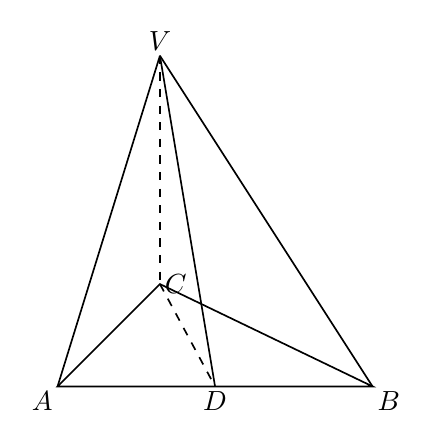
\begin{tikzpicture}[scale=1.0, semithick,
  every node/.style={inner sep=1.5pt}]
  \coordinate (A) at (0,0);
  \coordinate (B) at (4.0,0);
  \coordinate (C) at (1.3,1.3);
  \coordinate (V) at (1.3,4.2);
  \coordinate (D) at (2.0,0);

  \draw (A) -- (B) -- (C) -- cycle;
  \draw (V) -- (A);
  \draw (V) -- (B);
  \draw[dashed] (V) -- (C);
  \draw (V) -- (D);
  \draw[dashed] (C) -- (D);

  \node[below left] at (A) {$A$};
  \node[below right] at (B) {$B$};
  \node[right] at (C) {$C$};
  \node[above] at (V) {$V$};
  \node[below] at (D) {$D$};
\end{tikzpicture}
